\documentclass{math}

\usepackage{enumerate}
\usepackage{graphicx}

\title{Intro to Computer Science Theory: Homework 9}
\author{Alvin Lin and Joshua Cotton}
\date{August 2017 - December 2017}

\begin{document}

\maketitle

\subsection*{Problem 1}
Give CFGs for the following languages.
\begin{enumerate}[(a)]
  \item \( \{a^ib^jc^k\mid i=j~or~j=k\} \). \( G = (V,\Sigma,R,S) \)
  \begin{itemize}
    \item \( V = \{S,S_1,S_2,T_1,T_2,U_1,U_2\} \)
    \item \( \Sigma = \{a,b,c\} \)
    \item \( R = \{ \)
    \begin{itemize}
      \item \( S \to S_1\mid S_2 \)
      \item \( S_1 \to T_1U_1 \)
      \item \( T_1 \to aT_1b\mid\epsilon \)
      \item \( U_1 \to cU_1\mid\epsilon \)
      \item \( S_2 \to T_2U_2 \)
      \item \( T_2 \to uT_2\mid\epsilon \)
      \item \( U_2 \to bU_2c\mid\epsilon \)
    \end{itemize}
    \( \} \)
  \end{itemize}
  \item \( \{a^ib^{i+j}c^j\mid i\ge0~and~j\ge0\} \). \( G = (V,\Sigma,R,S) \)
  \begin{itemize}
    \item \( V = \{S,T,U\} \)
    \item \( \Sigma = \{a,b,c\} \)
    \item \( R = \{S\to TU, T\to\epsilon,T\to aTb,U\to\epsilon,U\to bUc\} \)
  \end{itemize}
  \item \( \{a^{i+j}b^ic^j\mid i\ge0~and~j\ge0\} \). \( G = (V,\Sigma,R,S) \)
  \begin{itemize}
    \item \( V = \{S,T\} \)
    \item \( \Sigma = \{a,b,c\} \)
    \item \( R = \{S\to aSc, S\to T, T\to aTb, T\to\epsilon\} \)
  \end{itemize}
\end{enumerate}

\subsection*{Problem 2}
Give state transition diagrams for PDAs for the following languages.
\begin{enumerate}[(a)]
  \item \( \{x\in\{a,b\}^*\mid n_a(x) = n_b(x)\} \)
  \begin{center}
    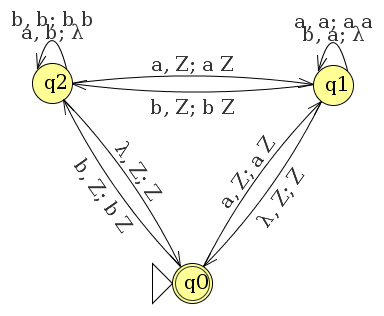
\includegraphics[width=8cm]{assets/hw_9_2a.png}
  \end{center}
  where \( Z \) denotes the empty stack character.
  \item \( \{x\in\{a,b\}^*\mid n_b(x)\le n_a(x)\le 2n_b(x)\} \)
  \[ ? \]
  \item The set of all balanced parentheses.
  \begin{center}
    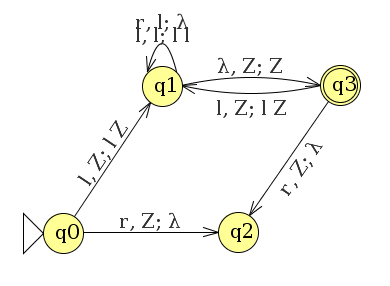
\includegraphics[width=8cm]{assets/hw_9_2c.png}
  \end{center}
  where \( Z \) denotes the empty stack character.
\end{enumerate}

\begin{center}
  If you have any questions, comments, or concerns, please contact me at
  alvin@omgimanerd.tech
\end{center}

\end{document}
